\documentclass{beamer}
\title{xv6 x86 \\ Scheduling}
\usetheme{CambridgeUS}
\usecolortheme{beaver}
\usepackage{kotex}
\usepackage{graphics}
\usepackage{booktabs}
\usepackage{listings}
\usepackage{local_dir}
\graphicspath{ {\rcufigure/xv6_scheduling/}}
\lstset{inputpath=\rcucode/xv6_scheduling/,
  basicstyle=\scriptsize,
  numbers=left,
  xleftmargin=10pt,
  tabsize=2,
}
\author{Chang-Hui Kim}

\begin{document}

\begin{frame}
  \titlepage
\end{frame}

%% -------------------------------------------------------------------------

\section{Multiplexing}

%% -------------------------------------------------------------------------

\begin{frame}[t]
  \frametitle{Multiplexing}
  Xv6 multiplexes by switching each processor from one process to another in two situations.

  \begin{itemize}
  \item \texttt{sleep} and \texttt{wakeup} mechanism.\\
    a process waits for
    \begin{itemize}
    \item device or pipe I/O to complete
    \item a child to exit
    \item or in sleep sys call
    \end{itemize}
  \item xv6 periodically forces a switch when a process is executing user instructions.
  \end{itemize}
  
\end{frame}

%% -------------------------------------------------------------------------

\begin{frame}[t]
  \frametitle{Challenges}
  Implementing multiplexing poses a few challenges.

  \begin{itemize}
  \item how to switch from one process to another?
  \item how to switch transparently to user processes?
  \item many CPUs may be switching among processes concurrently and a locking plan
    is necessary to avoid races.
  \item a process's memory and other resources must be freed when the process exits.
  \item each core of a multi-core machine must remember which process is
    executing so that system calls affect the correct process's kernel state.
  \end{itemize}
  
\end{frame}

%% -------------------------------------------------------------------------

\subsection{Code: Context switching}

%% -------------------------------------------------------------------------

\begin{frame}[t]
  \frametitle{Code: Context switching}

  \begin{figure}[ht]
    \centering
    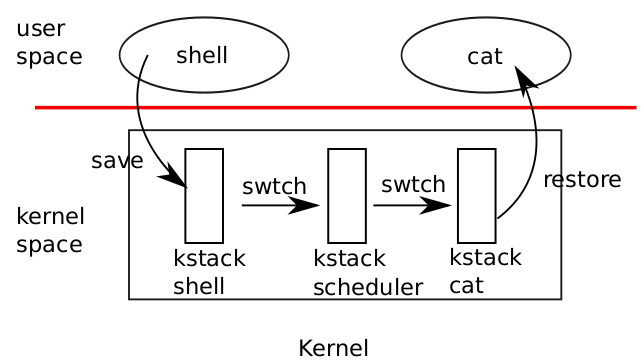
\includegraphics[width=0.6\textwidth]{fig5-1.png}
    \caption{Switching from one user process to another.
      In this example, xv6 runs with one CPU.}
  \end{figure}
  
\end{frame}

%% -------------------------------------------------------------------------

\begin{frame}[t]
  \frametitle{Code: Context switching}

  \begin{figure}[ht]
    \centering
    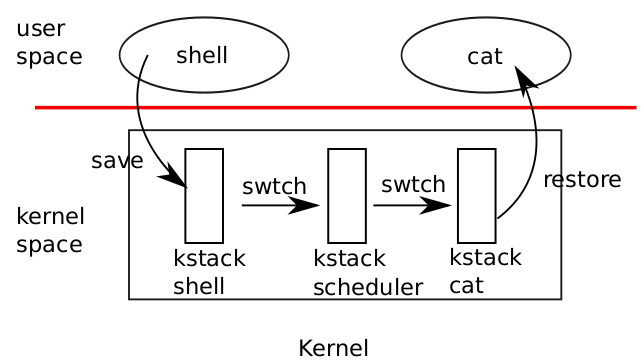
\includegraphics[width=0.4\textwidth]{fig5-1.png}
  \end{figure}

  \begin{enumerate}
  \item a user-kernel transition (system call or interrupt) to the old process’s kernel thread.
  \item a context switch to the current CPU’s scheduler thread.
  \item a context switch to a new process’s kernel thread.
  \item a trap return to the user-level process.
  \end{enumerate}
  
\end{frame}

%% -------------------------------------------------------------------------

\begin{frame}[t]
  \frametitle{Code: Context switching}
  The xv6 scheduler has its own thread (saved registers and stack) because it is sometimes not
  safe for it execute on any process’s kernel stack
  
\end{frame}

%% -------------------------------------------------------------------------

\begin{frame}[t]
  \frametitle{Code: Context switching}
  \begin{itemize}
  \item The function \texttt{swtch} performs the saves and restores for a thread switch.
  \item It just saves and restores register sets, called \texttt{contexts}.
  \end{itemize}

  \begin{figure}
    \lstinputlisting[basicstyle=\footnotesize]{struct_context.c}
    \caption{\texttt{struct context}}
  \end{figure}
  
\end{frame}

%% -------------------------------------------------------------------------

\begin{frame}[t]
  \frametitle{Code: Context switching}
  When it is time for a process to give up the CPU,
  \begin{enumerate}
  \item The process’s kernel thread calls \texttt{swtch}.
  \item \texttt{swtch} takes two arguments: \texttt{struct context **old} and \texttt{struct context *new}.
  \item It pushes the current registers onto the stack and saves the stack pointer in \texttt{*old}.
  \item Then swtch copies new to \texttt{\%esp}, pops previously saved registers, and returns.
  \item Each context is represented by a struct context*, a pointer to a structure stored on the kernel stack involved.
  \end{enumerate}

\end{frame}

%% -------------------------------------------------------------------------

\begin{frame}[t]
  \frametitle{Code: Context switching}
  \lstinputlisting[
    firstline=15, lastline=15, basicstyle=\footnotesize
  ]{sched.c}

  \begin{enumerate}
  \item Copying its arguments from the stack to the caller-saved registers \texttt{\%eax} and \texttt{\%edx}.
  \item \texttt{swtch} pushes the register state, creating a context structure on the current stack.
  \item Only the callee-saved registers need to be saved.
    \begin{enumerate}
    \item Pushes \texttt{\%ebp, \%ebx, \%esi, \%edi} explicitly.
    \item saves \texttt{\%esp} implicitly.
    \item \texttt{\%eip} has already been saved on the stack by the call instruction.
    \end{enumerate}
  \end{enumerate}
  
\end{frame}

%% -------------------------------------------------------------------------

\begin{frame}[t]
  \frametitle{Code: Context switching}
  Having saved the old context, \texttt{swtch} is ready to restore the new one.
  The new stack has the same form as the old one that \texttt{swtch} just left.
  \begin{enumerate}
  \item moves the pointer to the new context into the stack pointer.
  \item pops the values.
  \item then returns.
  \end{enumerate}
  
\end{frame}

%% -------------------------------------------------------------------------

\subsection{Code: Scheduling}

%% -------------------------------------------------------------------------

\begin{frame}[t]
  \frametitle{Code: Scheduling}

  Examine switching from a process through the scheduler to another process.\\
  A process that wants to give up the CPU
  \begin{itemize}
  \item must acquire the process table lock \texttt{ptable.lock}.
  \item release any other locks it is holding.
  \item update its own state. (\texttt{proc->state})
  \item then call \texttt{sched}.
  \end{itemize}

\end{frame}

%% -------------------------------------------------------------------------

\begin{frame}[t]
  \frametitle{Code: Scheduling}
  \texttt{sched} double-checks those conditions and then an implication of those conditions:\\
  Since a lock is held, the CPU should be running with interrupts disabled.

  \begin{figure}
    \lstinputlisting[
      firstline=5, lastline=13,
      basicstyle=\footnotesize]{sched.c}
  \end{figure}

  %% 1. check lock
  %% 2. check interrupt disabled
  %% 3. check process state
  %% 4. double check interrupt disabled
  
\end{frame}

%% -------------------------------------------------------------------------

\begin{frame}[t]
  \frametitle{Code: Scheduling}
  Finally, \texttt{sched} calls \texttt{swtch} to save the current context in
  \texttt{proc->context} and switch to the scheduler context in \texttt{cpu->scheduler}.

  \begin{figure}
    \lstinputlisting[
      firstline=14,
      lastline=17,
      basicstyle=\footnotesize
    ]{sched.c}
  \end{figure}

  \texttt{swtch} returns on the scheduler’s stack as though scheduler’s \texttt{swtch} had returned.
  
\end{frame}

%% -------------------------------------------------------------------------

\begin{frame}[t]
  \frametitle{Code: Scheduling}
  We just saw that xv6 holds ptable.lock across calls to swtch:

  \begin{itemize}
  \item The caller of \texttt{swtch} must already hold the lock
  \item Control of the lock passes to the switched-to code.
  \item \texttt{ptable.lock} protects
    \begin{itemize}
    \item invariants on the process's state.
    \item context fields that are not true while executing in \texttt{swtch}.
    \end{itemize}
  \end{itemize}
  
\end{frame}

%% -------------------------------------------------------------------------

\begin{frame}[t]
  \frametitle{Code: Scheduling}
  There is one case when the scheduler's call to swtch does not end up in sched.\\
  It begins at \texttt{forkret}.
  \begin{itemize}
  \item \texttt{forkret} exists to release the \texttt{ptable.lock}.
  \item The new process could start at \texttt{trapret}.
  \end{itemize}
  
\end{frame}

%% -------------------------------------------------------------------------

\begin{frame}[t]
  \frametitle{Code: Scheduling}
  Scheduler runs a simple loop:
  \begin{enumerate}
  \item find a process to run.
  \item run it until it yields.
  \item repeat.
  \end{enumerate}
  
\end{frame}

%% -------------------------------------------------------------------------

\begin{frame}[t]
  \frametitle{Code: Scheduling}
  \texttt{scheduler} releases the lock (and explicitly enables interrupts) once in each iteration of its outer loop.\\
  This is important for the special case in which this CPU is idle.

  \begin{enumerate}
  \item If an idling scheduler looped with the lock continuously held
  \item No other CPU that was running a process could ever perform
    \begin{itemize}
    \item a context switch.
    \item any process-related system call.
    \item in particular could never mark a process as \textbf{RUNNABLE}.
    \end{itemize}
  \end{enumerate}
  
\end{frame}

%% -------------------------------------------------------------------------

\begin{frame}[t]
  \frametitle{Code: Scheduling}
  The reason to enable interrupts periodically on an idling CPU is

  \begin{itemize}
  \item There is no RUNNABLE process because processes are waiting for I/O.
  \item If the scheduler left interrupts disabled all the time, the I/O would never arrive.
  \end{itemize}
  
\end{frame}

%% -------------------------------------------------------------------------

\begin{frame}[t]
  \frametitle{Invariant}
  If a process is 
  \begin{itemize}
  \item RUNNING, a timer interrupt's yield must be able to switch away from the process.
  \item RUNNABLE, an idle CPU’s scheduler must be able to run it.
  \end{itemize}

\end{frame}

%% -------------------------------------------------------------------------

\begin{frame}[t]
  \frametitle{Invariant}
  Once the code has started to modify a running process's state to make it RUNNABLE
  \begin{itemize}
  \item It must hold the lock until it has finished restoring the invariants.
  \item The earliest correct release point is after \texttt{scheduler} stops using the process's page table and clears proc.
  \end{itemize}
\end{frame}

%% -------------------------------------------------------------------------

\begin{frame}[t]
  \frametitle{Invariant}
  Once scheduler starts to convert a runnable process to RUNNING
  \begin{itemize}
  \item The lock cannot be released until the kernel thread is completely running.
  \item after the \texttt{swtch}, e.g. in \texttt{yield}.
  \end{itemize}
  
\end{frame}

%% -------------------------------------------------------------------------

\begin{frame}[t]
  \frametitle{\texttt{ptable.lock}}
  \texttt{ptable.lock} protects other things as well:
  \begin{itemize}
  \item allocation of process IDs.
  \item free process table slots.
  \item the interplay between \texttt{exit} and \texttt{wait}.
  \item the machinery to avoid lost wakeups (see next section).
  \end{itemize}
  
\end{frame}

%% -------------------------------------------------------------------------

\subsection{Code: mycpu and myproc}

%% -------------------------------------------------------------------------

\begin{frame}[t]
  \frametitle{Code: mycpu and myproc}

  xv6 maintains a \texttt{struct cpu} for each processor
  \begin{itemize}
  \item The processor's unique hardware identifier (\texttt{apicid})
  \item Records the process currently running on the processor
  \end{itemize}

  \begin{figure}
    \lstinputlisting[firstline=1, lastline=11,
      basicstyle=\footnotesize]{sched.h}
  \end{figure}
  
\end{frame}

%% -------------------------------------------------------------------------

\begin{frame}[t]
  \frametitle{Code: mycpu and myproc}
  The function \texttt{mycpu} returns the current processor's \texttt{struct cpu}.

  \begin{enumerate}
  \item reading the processor identifier from the local APIC hardware.
  \item looking through the array of \texttt{struct cpu} for an entry with that identifier.
  \end{enumerate}
  
\end{frame}

%% -------------------------------------------------------------------------

\begin{frame}[t]
  \frametitle{Code: mycpu and myproc}
  The return value of \texttt{mycpu} is fragile. 

  \begin{itemize}
  \item xv6 requires that callers of \texttt{mycpu} disable interrupts.
  \item only enable them after they finish using the returned \texttt{struct cpu}.
  \end{itemize}
  
\end{frame}

%% -------------------------------------------------------------------------

\begin{frame}[t]
  \frametitle{Code: mycpu and myproc}
  The function \texttt{myproc} returns the \texttt{struct proc} pointer for the process
  that is running on the current processor.

  \begin{enumerate}
  \item disables interrupts.
  \item invokes \texttt{mycpu}.
  \item fetches the current process pointer (\texttt{c->proc}) out of the
    \texttt{struct cpu}.
  \item enables interrupts.
  \end{enumerate}
  
\end{frame}

%% -------------------------------------------------------------------------

\begin{frame}[t]

  \frametitle{Code: mycpu and myproc}
  \begin{itemize}
  \item If there is no process running, because the the caller is executing in \texttt{scheduler},
    \texttt{myproc} returns zero.
  \item The return value of \texttt{myproc} is safe to use even if interrupts are enabled.
  \end{itemize}
  
\end{frame}

%% -------------------------------------------------------------------------

\section{Sleep and wakeup}

%% -------------------------------------------------------------------------

\begin{frame}[t]
  \frametitle{Sleep and wakeup}
  So far we have no abstractions that help processes intentionally interact.\\
  \begin{center}
    Sleep and wakeup fill that void, allowing one process to sleep waiting for an
    event and another process to wake it up once the event has happened.
  \end{center}
  
\end{frame}

%% -------------------------------------------------------------------------

\begin{frame}[t]
  \frametitle{Sleep and wakeup}
  \begin{columns}
    \begin{column}{.5\textwidth}
      \lstinputlisting[firstline=45, lastline=51, basicstyle=\footnotesize]
                      {sleep_wait.c}
    \end{column}
    \begin{column}{.425\textwidth}
      \lstinputlisting[firstline=53, lastline=61, basicstyle=\footnotesize]
                      {sleep_wait.c}
    \end{column}
  \end{columns}
  
\end{frame}

%% -------------------------------------------------------------------------

\begin{frame}[t]
  \frametitle{Sleep and wakeup}
  \begin{figure}[ht]
    \centering
    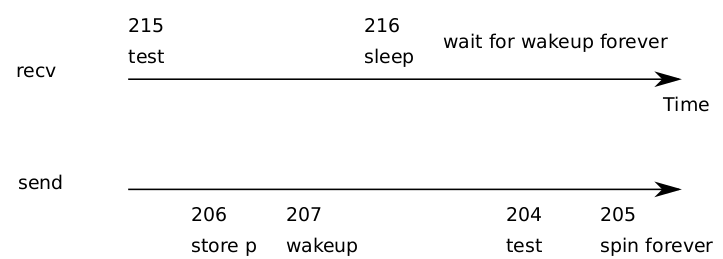
\includegraphics[width=0.9\textwidth]{fig5-2.png}
    \caption{Example lost wakeup problem}
  \end{figure}

  \texttt{recv} sleeps when \texttt{q->ptr == 0} violated by \texttt{send}.
  
\end{frame}

%% -------------------------------------------------------------------------

\begin{frame}[t]
  \frametitle{Sleep and wakeup}
  \begin{columns}
    \begin{column}{.5\textwidth}
      \lstinputlisting[firstline=1, lastline=9, basicstyle=\footnotesize]
                      {sleep_wait.c}
    \end{column}
    \begin{column}{.425\textwidth}
      \lstinputlisting[firstline=11, lastline=21, basicstyle=\footnotesize]
                      {sleep_wait.c}
    \end{column}
  \end{columns}

  \texttt{recv} holds the lock while it sleeps, so the sender will block
  forever waiting for the lock.
  
\end{frame}

%% -------------------------------------------------------------------------

\begin{frame}[t]
  \frametitle{Sleep and wakeup}
  \begin{columns}
    \begin{column}{.5\textwidth}
      \lstinputlisting[firstline=23, lastline=31, basicstyle=\footnotesize]
                      {sleep_wait.c}
    \end{column}
    \begin{column}{.425\textwidth}
      \lstinputlisting[firstline=33, lastline=43, basicstyle=\footnotesize]
                      {sleep_wait.c}
    \end{column}
  \end{columns}
  changing \texttt{sleep}'s interface:
  \begin{itemize}
  \item pass the lock to sleep so it can release the lock
  \item awake again \texttt{sleep} reacquires the lock before returning.
  \end{itemize}
  
\end{frame}

%% -------------------------------------------------------------------------

\begin{frame}[t]
  \frametitle{Sleep and wakeup}

  \begin{itemize}
  \item \texttt{recv} holds \texttt{q->lock} prevents \texttt{send} from trying to wake
    it up between \texttt{recv}'s check of \texttt{q->ptr} and its call to \texttt{sleep}.
  \item need \texttt{sleep} to atomically release \texttt{q->lock} and put the receving
    process to sleep.
  \end{itemize}
  
\end{frame}

%% -------------------------------------------------------------------------

\subsection{Code: Sleep and wakeup}

%% -------------------------------------------------------------------------

\begin{frame}[t]
  \frametitle{The basic idea}
  \texttt{sleep}
  \begin{enumerate}
  \item mark the current process as \texttt{SLEEPING}.
  \item call \texttt{sched} to release the processor.
  \end{enumerate}

  \texttt{wakeup}
  \begin{enumerate}
  \item looks for a process sleeping on the given wait channel.
  \item marks it as \texttt{RUNNABLE}.
  \end{enumerate}
  

\end{frame}

%% -------------------------------------------------------------------------

\begin{frame}[t]
  \frametitle{Usage}

  \begin{itemize}
  \item Callers of sleep and wakeup can use any mutually convenient number as the channel.
  \item Xv6 often uses the address of a kernel data structure involved in the waiting.
  \end{itemize}
  
\end{frame}

%% -------------------------------------------------------------------------

\begin{frame}[t]
  \frametitle{How does \texttt{sleep} work}

  \texttt{sleep} begins with a few sanity checks:
  \begin{itemize}
  \item there must be a current process.
  \item \texttt{sleep} must have been passed a lock.
  \end{itemize}
  
\end{frame}

%% -------------------------------------------------------------------------

\begin{frame}[t]
  \frametitle{How does \texttt{sleep} work}

  acquires \texttt{ptable.lock}.
  \begin{itemize}
  \item ensured that no other process could start a call to \texttt{wakeup}.
  \item safe to release \texttt{lk}.
    \begin{itemize}
    \item some other process start a call to \texttt{wakeup}, \texttt{wakeup} will not
      run until it can acquire \texttt{ptable.lock}.
    \item keeping the \texttt{wakeup} from missing the \texttt{sleep}.
    \end{itemize}
  \end{itemize}

  \begin{center}
    if \texttt{ptable.lock} is equal to \texttt{lk}, then skip acquiring.
  \end{center}
  
\end{frame}

%% -------------------------------------------------------------------------

\begin{frame}[t]
  \frametitle{How does \texttt{wakeup} work}
  \begin{enumerate}
  \item acquire \texttt{ptable.lock}.\\
    because
    \begin{itemize}
    \item manipulating process states.
    \item \texttt{sleep} and \texttt{wakeup} do not miss each other.
    \end{itemize}
  \item call \texttt{wakeup1}.
    \begin{enumerate}
    \item search for a process in state \texttt{SLEEPING} with a matching \texttt{chen}.
    \item changes it's state to \texttt{RUNNABLE}.
    \end{enumerate}
  \end{enumerate}
  
\end{frame}

%% -------------------------------------------------------------------------

\begin{frame}[t]
  \frametitle{Guard the sleep condition}

  Xv6 code always calls \texttt{wakeup} while holding the lock that guards
  the sleep condition.

  \begin{center}
    Why do the locking rules for sleep and wakeup ensure a sleeping process won’t miss
    a wakeup it needs?
  \end{center}
  
\end{frame}

%% -------------------------------------------------------------------------

\begin{frame}[t]
  \frametitle{Guard the sleep condition}

  If a concurrent thread causes the condition to be true, that thread
  must either hold the lock on the condition.

  \begin{itemize}
  \item before sleep thread acquire condition lock.
  \item after sleep thread acquire condition lock.
  \end{itemize}

  %% When before sleep thread acquire condition lock, eventhough,
  %% the sleep thread goto sleep, it is intended behavior. Because
  %% the sleep thread knows the condition is true. (Intended behavior)
  
\end{frame}

%% -------------------------------------------------------------------------

\begin{frame}[t]
  \frametitle{Guard the sleep condition}

  \begin{figure}[ht]
    \centering
    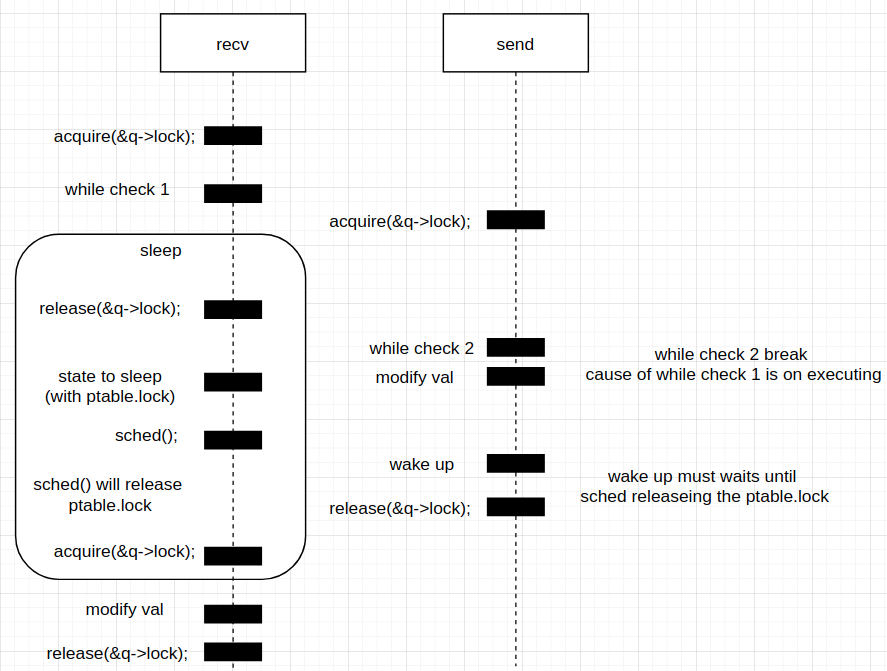
\includegraphics[width=0.8\textwidth]{after_acq.png}
  \end{figure}

  %% if start sleep function, sleep process is critical section.

\end{frame}

%% -------------------------------------------------------------------------

\begin{frame}[t]
  \frametitle{Guard the sleep condition}

  \begin{center}
    while loop is need.
  \end{center}

  \begin{itemize}
  \item A single call to wakeup will wake them all up.
  \item No harm is done if two uses of sleep/wakeup accidentally choose the same channel.
  \end{itemize}
  
\end{frame}

%% -------------------------------------------------------------------------

\subsection{Code: Pipes}

%% -------------------------------------------------------------------------

\begin{frame}[t]
  \frametitle{Code: Pipes}

  \lstinputlisting[firstline=42, lastline=49, basicstyle=\tiny]{pipe.c}

  \begin{itemize}
  \item \texttt{nread} and \texttt{nwrite} count the number of bytes read from and written
    to the buffer.
  \item buffer: circular queue
  \item The counts do not wrap. % normally nread != nwrite
  \item a full buffer (\texttt{nwrite == nread+PIPESIZE})
  \item an empty buffer (\texttt{nwrite == nread})
  \end{itemize}
  
\end{frame}

%% -------------------------------------------------------------------------

\begin{frame}[t]
  \frametitle{Code: Pipes}

  \lstinputlisting[firstline=21, lastline=40, basicstyle=\tiny]{pipe.c}
  
\end{frame}

%% -------------------------------------------------------------------------

\begin{frame}[t]
  \frametitle{Code: Pipes}

  \lstinputlisting[firstline=1, lastline=19, basicstyle=\tiny]{pipe.c}
  
   The pipe code uses separate sleep channels for reader and writer
\end{frame}

%% -------------------------------------------------------------------------

\subsection{Code: Wait, exit, and kill}

%% -------------------------------------------------------------------------

\begin{frame}[t]
  \frametitle{Code: Wait, exit}

  When a child exits,
  \begin{itemize}
  \item It switches to the \texttt{ZOMBIE} process state until the parent
    calls \texttt{wait}.
  \item The parent is then responsible for
    \begin{itemize}
    \item freeing the memory associated with the process.
    \item preparing the \texttt{struct proc} for reuse.
    \end{itemize}
  \item If the parent exits before the child, the init process adopts
    the child and waits for it.
  \end{itemize}
  
\end{frame}

%% -------------------------------------------------------------------------

\begin{frame}[t]
  \frametitle{Code: Wait}

  \begin{enumerate}
  \item \texttt{wait} begins by acquiring \texttt{ptable.lock}.
  \item scans the process table looking for children.
  \item If wait finds that the current process has children but that none have exited,
    \begin{enumerate}
    \item It calls sleep to wait for one of them to exit.
    \item scans again.
    \end{enumerate}
  \end{enumerate}
  
\end{frame}

%% -------------------------------------------------------------------------

\begin{frame}[t]
  \frametitle{Code: Exit}

  \begin{enumerate}
  \item \texttt{exit} acquires \texttt{ptable.lock}.
  \item wakes up any process sleeping on a wait
    channel equal to the current process’s parent proc
  \item set its state to \texttt{ZOMBIE}.
  \item reparents all of the exiting process’s children,
    passing them to the \texttt{initproc}.
  \item calls \texttt{sched} to relinquish the CPU.
  \end{enumerate}

  \begin{center}
    although \texttt{wakeup} may cause the parent to run, the loop in wait cannot run until
    \texttt{exit} releases \texttt{ptable.lock}.
  \end{center}

\end{frame}

%% -------------------------------------------------------------------------

\begin{frame}[t]
  \frametitle{Code: Wait}

  \begin{enumerate}
    \setcounter{enumi}{3}
  \item finds the exited child with \texttt{state == ZOMBIE}.
  \item records the child’s pid.
  \item cleans up the \texttt{struct proc}.
  \item freeing the memory associated with the process.
  \end{enumerate}
  
\end{frame}

%% -------------------------------------------------------------------------

\begin{frame}[t]
  \frametitle{Code: Kill}
  \begin{itemize}
  \item lets one process request that another be terminated.
  \item just sets the victim's \texttt{p->killed}. (Cause of complexity)
  \item if victim is sleeping, wakes it up.
  \end{itemize}

  \begin{center}
    The victim will enter or leave the kernel, at which point code in trap will call
    \texttt{exit} if \texttt{p->killed} is set.
  \end{center}
  
\end{frame}

%% -------------------------------------------------------------------------

\begin{frame}[t]
  \frametitle{Code: Kill}

  \begin{itemize}
  \item If the victim process is in \texttt{sleep}, the call to \texttt{wakeup} will
    cause the victim process to return from \texttt{sleep}.
  \item This is potentially dangerous because the condition being waiting
    for may not be true.
  \end{itemize}
  
\end{frame}

%% -------------------------------------------------------------------------

\begin{frame}[t]
  \frametitle{Code: Kill}
  xv6 calls to sleep are always wrapped in a while loop that re-tests the condition
  after \texttt{sleep} returns.
  \begin{itemize}
  \item Some calls to sleep also test \texttt{p->killed} in the loop,
    and abandon the current activity if it is set.
  \item Some xv6 sleep loops do not check \texttt{p->killed}.
  \end{itemize}

  \begin{center}
    To avoid the complication of cleaning up after a partial operation, xv6 delays
    the killing of a process
  \end{center}
  %% do properly depend on situation.
\end{frame}

\end{document}
